% !TEX root = rapport_root.tex
\section{Content Analysis with an Iterative LLM: Identifying Theories and Methods}

Once the articles were classified into section types, we were well-poised to
perform a more fine-grained analysis. Our goal was to move beyond broad topics
and identify the specific theoretical frameworks and research methods used
within the PRPER corpus, and to track how their usage has evolved over time. To
achieve this, we developed a novel, iterative classification workflow that uses
an LLM to discover and assign fine-grained categories directly from the text.

\subsection{Methodology: An Iterative Classification Workflow}

To extract specific information like theoretical frameworks, we developed a
staged, iterative approach that uses an LLM to build a classification scheme
from the ground up. As illustrated in Figures \ref{fig:classifier_logic} and
\ref{fig:classifier_workflow}, the process involves:
\begin{enumerate}
    \item Feeding a sample of text sections to an LLM to generate an initial
    list of categories.
    \item Using this list to classify all sections.
    \item Reviewing the classifications and having the LLM refine or merge the
    categories.
    \item Repeating the process until the classification scheme is stable and
    comprehensive.
\end{enumerate}
This logic is implemented in a flexible Python `AbstractClass`. A key feature of
this implementation is the format of the LLM's response. For each section, the
model returns both a direct array of classifications (e.g., the specific
frameworks it identifies) and a corresponding probability distribution. This
provides analytical flexibility, allowing us to either accept the model's direct
classifications, filter results by a confidence threshold, or select only the
single highest-probability result.

\begin{figure}
    \centering
    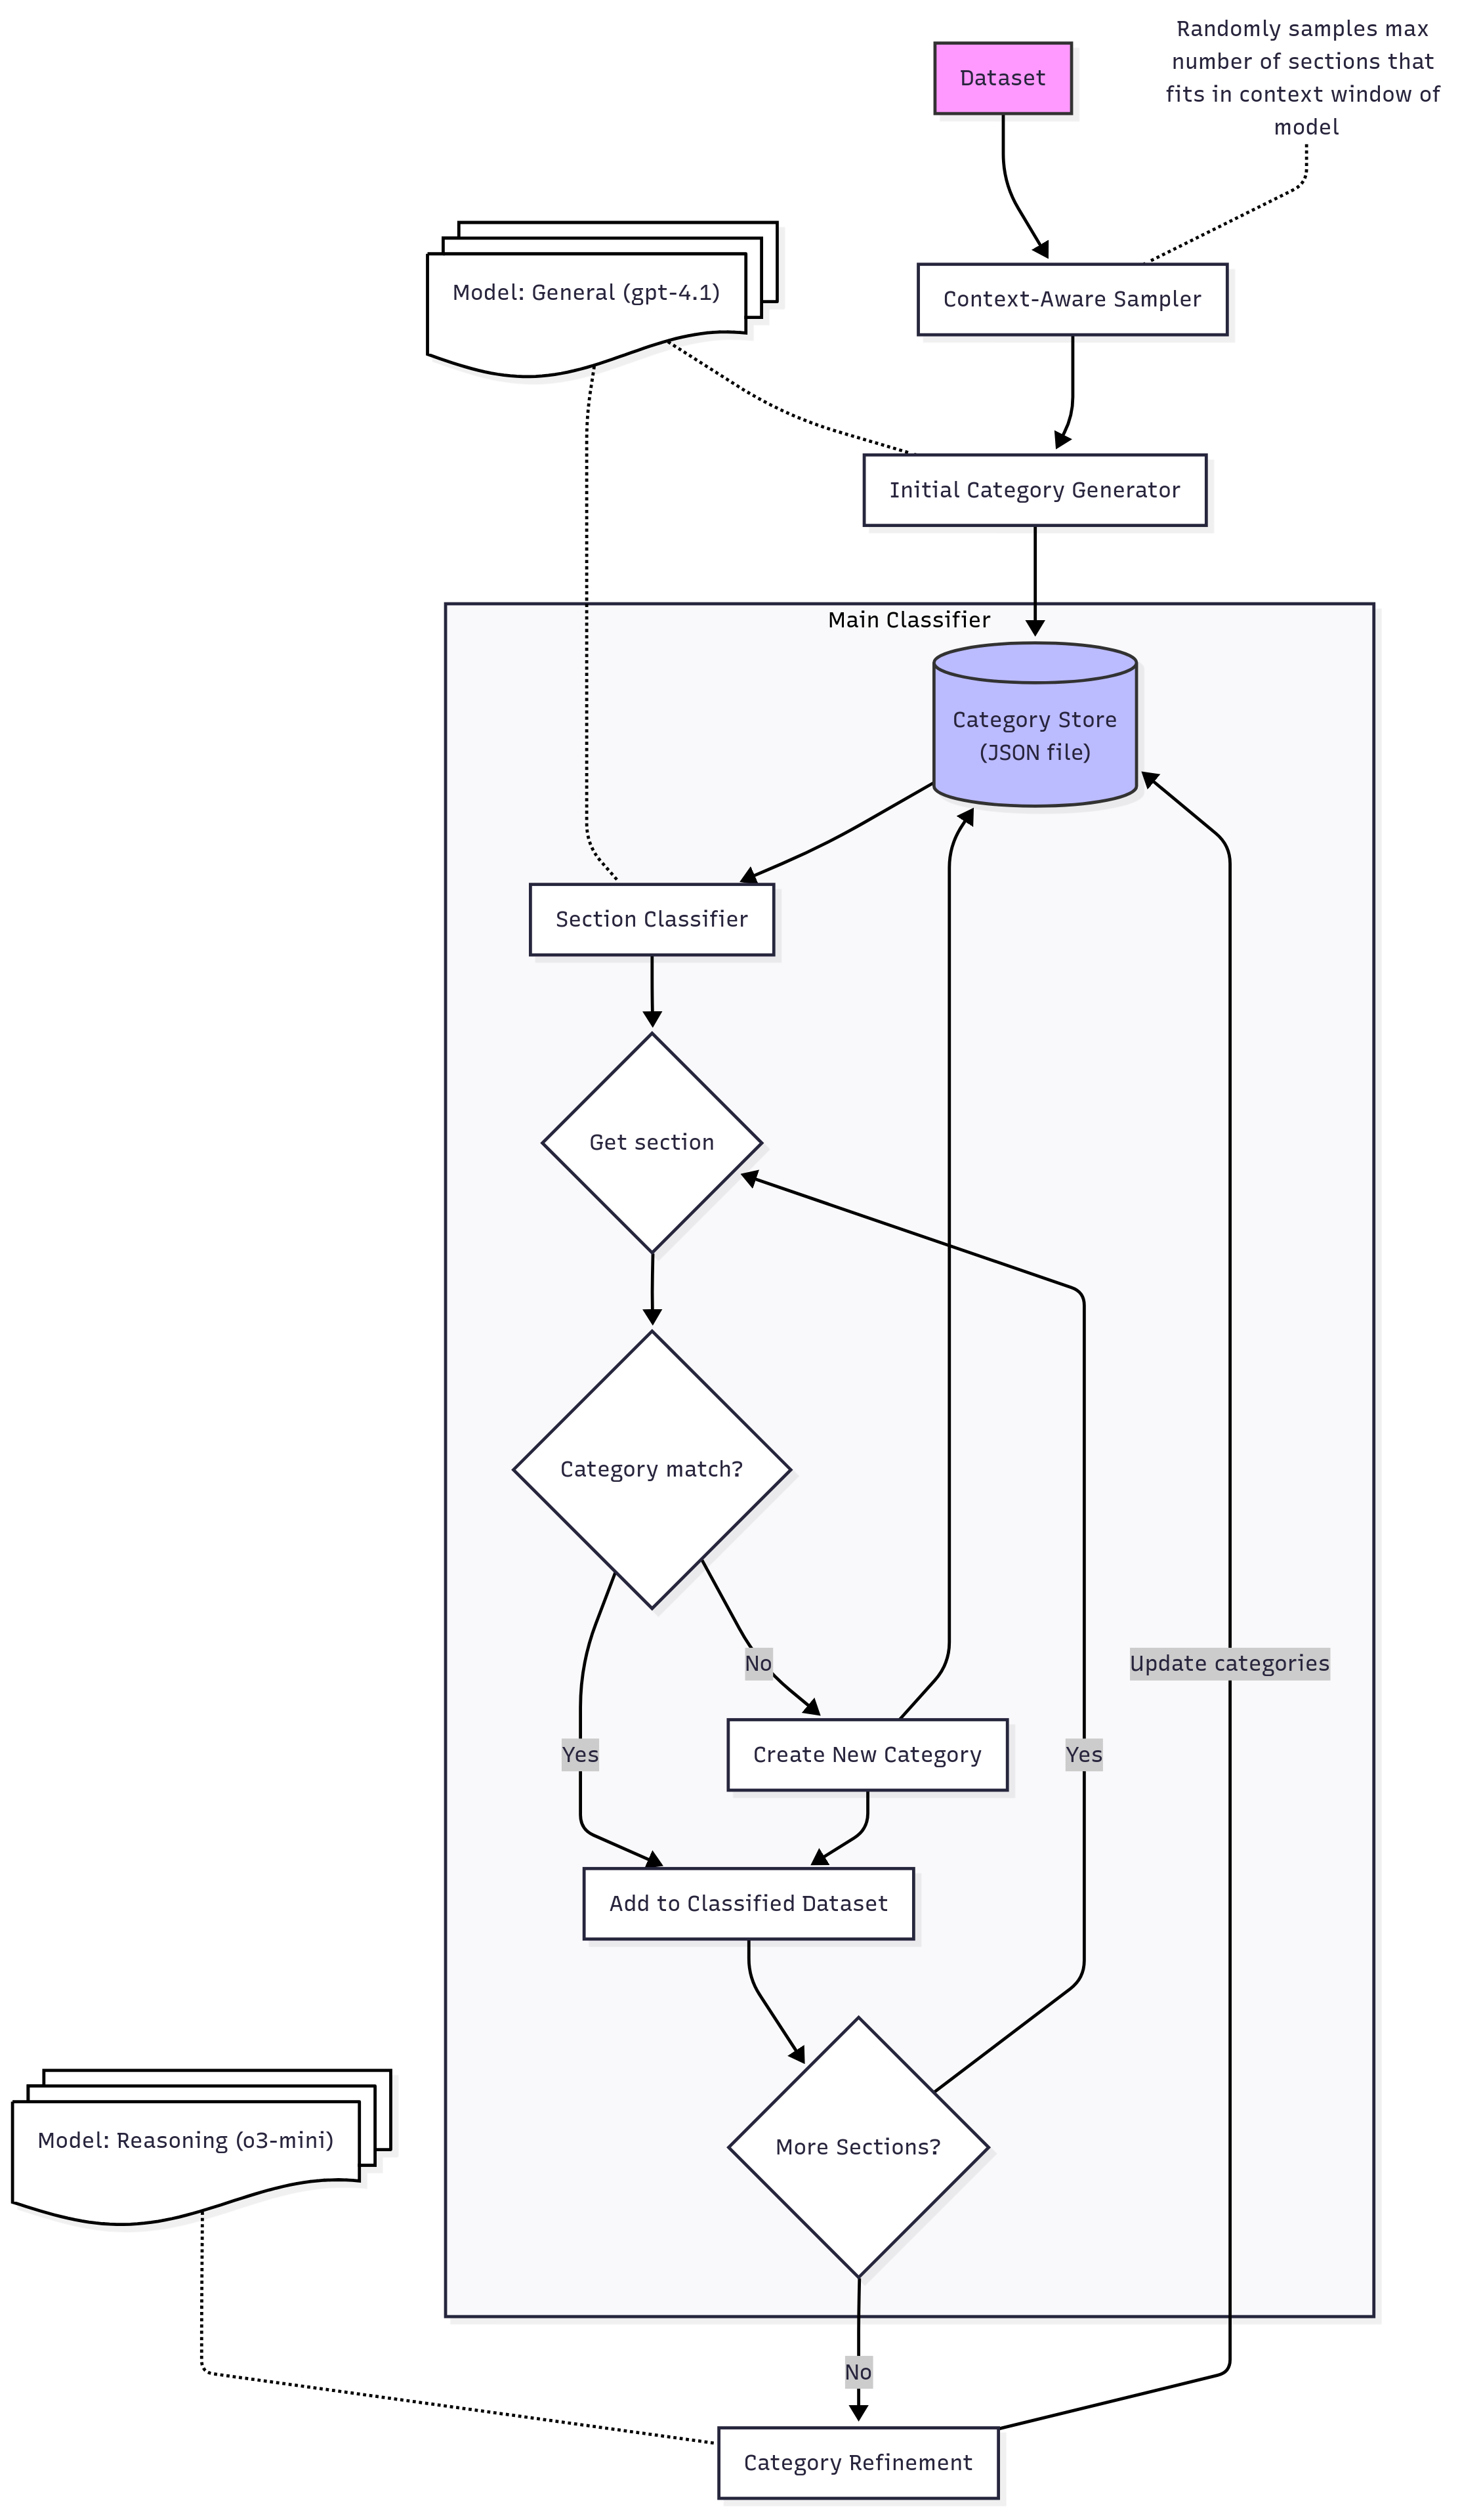
\includegraphics[width=0.7\textwidth]{media/classifier_logic.png}
    \caption{Abstract logic of the iterative LLM classifier.}
    \label{fig:classifier_logic}
\end{figure}

\begin{figure}
    \centering
    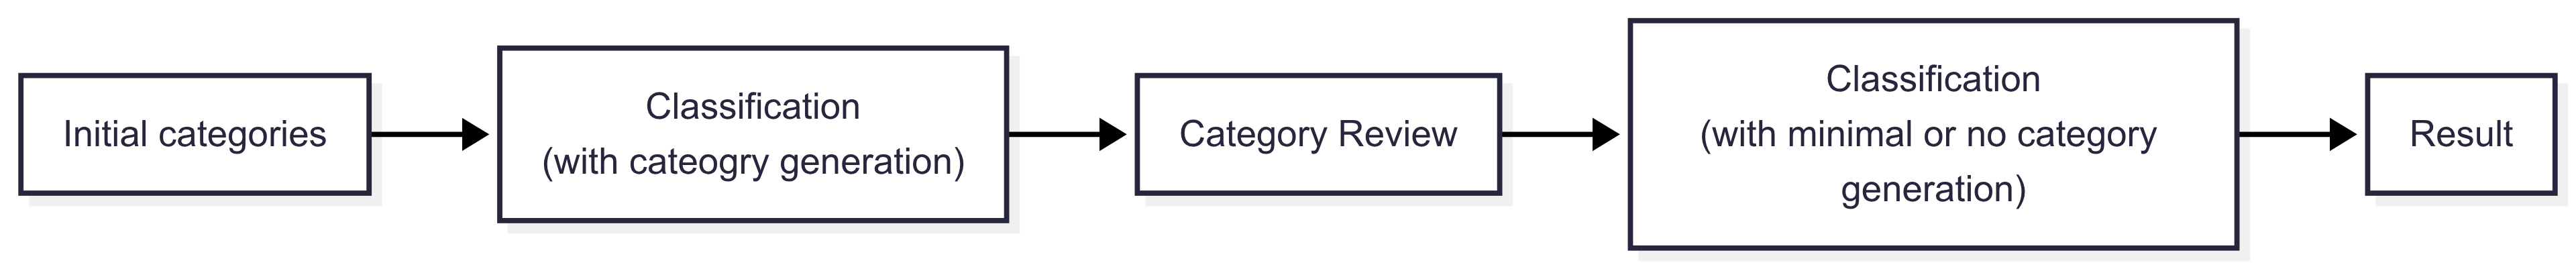
\includegraphics[width=0.7\textwidth]{media/general-workflow.png}
    \caption{General workflow of how we used the classifier to generate results.}
    \label{fig:classifier_workflow}
\end{figure}

\subsubsection{Identifying and Classifying Theoretical Frameworks}

We first applied this workflow to the 589 sections classified as `Theoretical
Framework`. The process generated a fine-grained list of 135 distinct
frameworks. To make this data more interpretable for trend analysis, we ran the
classifier on the framework list itself to group them into six meta-categories
(e.g., \emph{Cognitive, Sociocultural, Social Justice}). Using these
meta-categories, we were able to plot the evolution of theoretical interests in
PRPER over time, as shown in Figure~\ref{fig:theoretical_development}.

\begin{figure}
    \centering
    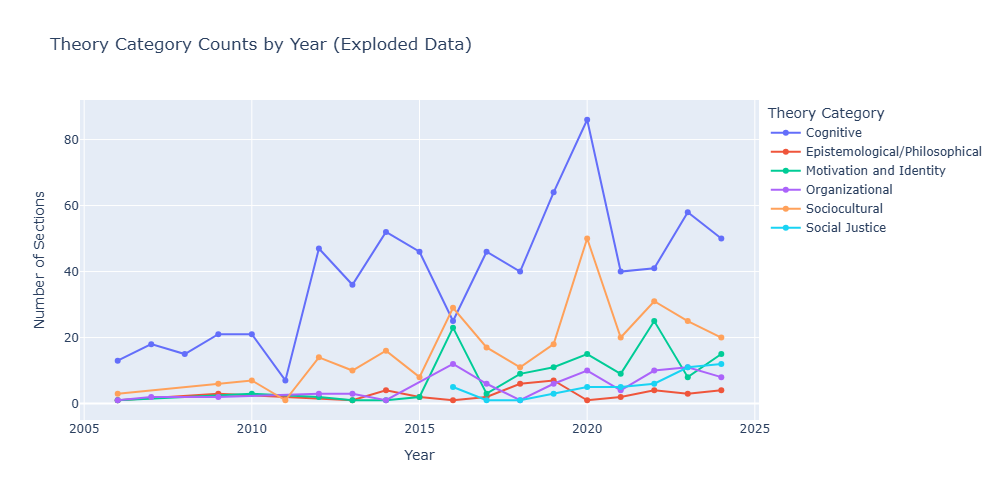
\includegraphics[width=0.7\textwidth]{media/theory_year_exploded.png}
    \caption{Theoretical developments in PRPER over time, grouped by meta-category.}
    \label{fig:theoretical_development}
\end{figure}

\subsubsection{Identifying and Classifying Methods}

We replicated the same process for all sections classified as `Methods`.
As we had no predefined meta-categories for research methods, we used the
classifier's automatic category generation feature to produce an initial list
for review. This allowed us to meta-categorize the identified methods and plot
their development over time.

\subsection{Discussion of the Iterative Classifier}

This iterative, LLM-based approach has several significant advantages. Rather
than relying on a predefined list, the classifier discovers emergent theoretical
and methodological categories directly from the corpus, making it a powerful
tool for large-scale, qualitative discovery. Furthermore, its implemented as a
flexible software framework. The classifier is built upon a set of abstract
Python classes that define the core iterative workflow. This design allows for
easy extension to new tasks; one can create a novel classifier, for example to
identify research questions, simply by inheriting from a base class and
providing new, task-specific prompts. The framework also uses Pydantic models to
ensure that all data exchanged with the LLM is structured and valid. For more
technical details, see the module's documentation.

However, the approach involves practical considerations and trade-offs. The
iterative process, which involves multiple chained calls to an LLM, can incur
monetary costs with APIs. As we noted earlier, running these tasks on powerful,
local open-source models would solve the cost and data privacy issues but
demands notable local computing resources. Furthermore, the "black box" nature
of LLMs means that the reasoning behind category creation is not always
transparent, and the process requires a human-in-the-loop to review and validate
the generated categories for quality and coherence.

A key challenge we noticed, particularly when classifying research methods, was
that the model sometimes struggled to distinguish between the \emph{use} of a
method versus the \emph{discussion} of one. For instance, some articles were
classified as employing both qualitative and quantitative methods. While time
constraints prevented a systematic manual review of these cases, we suspect that
an article can \emph{use} one approach while contrasting it with another; i.e.
the LLM can struggle to distunguish between \emph{use} and \emph{discussion} of
a method. This suggests the `gpt-4o-mini` model, while efficient, can lack the
nuance to grasp this contextual distinction. We hypothesize that using a more
powerful model could mitigate this issue, as it may be better at discerning an
author's primary methodology from the surrounding methodological discussion.

Despite these considerations, this method enables a novel form of automated
literature review, allowing for a fine-grained analysis of conceptual trends at
a scale that would be prohibitive to achieve manually.